\documentclass[11pt,a4paper]{article}
\usepackage[T1]{fontenc}
\usepackage{mathptmx}
\usepackage{amsmath,amssymb,amsthm}
\usepackage{geometry}
\usepackage[hidelinks]{hyperref}
\usepackage{booktabs}
\usepackage{graphicx}
\usepackage{xcolor}
\usepackage{listings}
\usepackage{enumitem}
\usepackage{url}
\graphicspath{{./figures/}{./}}
\geometry{margin=2.5cm}

\newtheorem{theorem}{Theorem}
\newtheorem{proposition}[theorem]{Proposition}
\newtheorem{lemma}[theorem]{Lemma}
\theoremstyle{definition}
\newtheorem{definition}{Definition}
\theoremstyle{remark}
\newtheorem{remark}{Remark}

\lstset{basicstyle=\ttfamily\small,frame=single,breaklines=true,language=Python,showstringspaces=false,columns=fullflexible}

\title{\textbf{Biological Transitions as Multi-Agent Realisations of the}\\
\textbf{Generative Operator Pipeline in Topographical Orthogonal}\\
\textbf{Generative Theory (TO/TOGT): A Fruit-Fly Connectome Toy Model}\\[0.5em]
\large\emph{Version 3 --- what the model does, and corrections}}

\author{Pablo Nogueira Grossi\\
G6 LLC, Newark, New Jersey, USA\\
ORCID: 0009-0000-6496-2186\\[0.3em]
\small Concept DOI: \href{https://doi.org/10.5281/zenodo.19210136}{10.5281/zenodo.19210136}
\quad V2: \href{https://doi.org/10.5281/zenodo.20128568}{10.5281/zenodo.20128568}
\quad V3: DOIPLACEHOLDER}

\date{March 2026 (v1); May 2026 (v2); September 2026 (v3 -- this revision)}

\begin{document}
\maketitle

\begin{abstract}
We study a toy model of a swarm of neural clusters, motivated by the \textit{Drosophila} connectome
\cite{Dorkenwald2024}. Each cluster is a point in the plane; one step applies the operator pipeline
$G=U\circ F\circ K\circ C$ of TO/TOGT (compress, clip, fold with a neighbour, rescale), with coupling
$\alpha$ to the next cluster in a ring. Version~2 stated that for $|\alpha|<\tfrac12$ the swarm map is a
contraction with Lipschitz constant $L(\alpha)=\tfrac12+|\alpha|$ and a unique fixed point, and that a
pitchfork bifurcation occurs at $|\alpha|=\tfrac12$. Version~3 shows that these statements do not hold: $G$ is
discontinuous, so it has no Lipschitz constant; a single agent already has four fixed points at $\alpha=0$;
and the quantity plotted as the bifurcation signature is fixed at $1$ by construction. We then measure what
the model does. It is \emph{multistable}: for weak coupling every run settles fast, and 40 random starts reach
40 different end states. Near the threshold the version~2 paper proposed, its behaviour changes: in our runs
the first cycles appear at $\alpha=0.42$, most runs cycle at $\alpha=0.5$--$0.65$, and from $\alpha=0.7$ some
runs neither settle nor repeat within 400 steps. The corrections are proved in Lean~4 (Mathlib v4.32.0) with no
\texttt{sorry}; the measurements are reproducible with the deposited code.
\end{abstract}

\noindent\textbf{Keywords:} TO/TOGT; operator pipeline; fruit-fly connectome; multi-agent dynamics;
multistability; coupled map lattice; Lean~4.\quad
\textbf{MSC:} 37C25, 37N25, 92B20.

\section{Relation to Prior Work}
This paper supplements \textit{Principia Orthogona, Volume One} \cite{Grossi2026_Vol1} and the broader
biological-transitions paper \cite{Grossi2026_MultiAgent}. The FlyWire connectome \cite{Dorkenwald2024,
Schlegel2024} and the larval connectome \cite{Winding2023} motivate the ring-of-clusters topology only; no
connectome data is fitted, and the model is not a quantitative neuroscience claim. Coupled systems of
identical units can show multistability and switching between rest and oscillation, as in the analysis of
coupled Hopf oscillators in perceptual bistability \cite{PerezCervera2019}. Bistable switching has also been
modelled in the hypothalamic--pituitary--adrenal (HPA) stress axis \cite{Zarzer2013}. Version~2 cited an HPA
paper (Bhaskaran \textit{et al.}, \textit{J.\ Theor.\ Biol.}\ 540, 111077, 2022) whose DOI is not registered
and which we could not find; it is withdrawn here.

\section{The Operator Pipeline}
\begin{definition}\label{def:G}
For an agent state $s=(x,y)\in\mathbb{R}^2$ and its neighbour's state $n$, one step is $G_\alpha(s;n)=U(F_\alpha(K_b(C(s)),n))$ with
\begin{itemize}[leftmargin=2em,itemsep=2pt]
\item $C$ (compress): keep the larger coordinate and set the other to $0$; $C(x,y)=(x,0)$ if $|y|\le|x|$, else $(0,y)$;
\item $K_b$ (clip): $K_b(s)=\mathrm{clip}(s+b\,\mathrm{sgn}(s),-1,1)$ coordinatewise, $b=0.1$, with $\mathrm{sgn}(0)=+1$ as in the code (\texttt{np.sign(s + 1e-12)});
\item $F_\alpha$ (fold): $F_\alpha(s,n)=(1-\alpha)s+\alpha n$;
\item $U$ (unfold): $U(s)=s/\|s\|$ for $s\neq0$.
\end{itemize}
The swarm is $N$ agents on a ring, $s_i^{t+1}=G_\alpha(s_i^t;s_{i+1}^t)$ (indices mod $N$). Version~2 added
Gaussian noise of size $\sigma=0.01$; all measurements below are noise-free.
\end{definition}

\begin{figure}[h]\centering
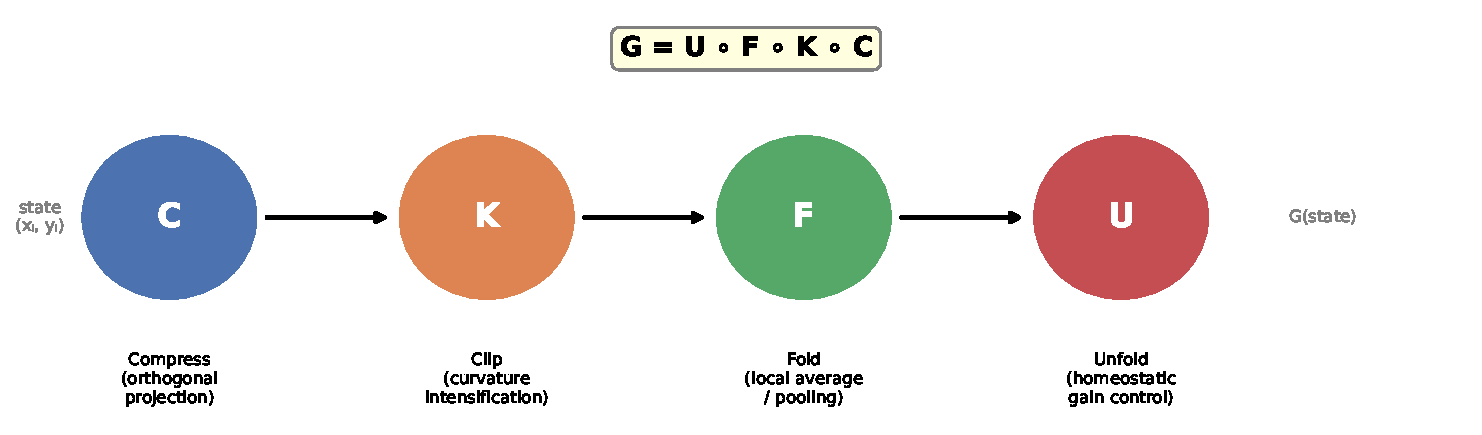
\includegraphics[width=0.95\linewidth]{fig4_operator_diagram}
\caption{Schematic of $G=U\circ F\circ K\circ C$ (from version 2).}\label{fig:pipeline}
\end{figure}

\section{What Does Not Hold}
\begin{proposition}[No Lipschitz constant]\label{prop:jump}
$C$ sends $(1,0.999)$ and $(0.999,1)$, which are $0.002$ apart in $\ell^1$, to $(1,0)$ and $(0,1)$, which are $2$
apart. Hence $C$ is discontinuous, and $G_\alpha$ has no Lipschitz constant for any $\alpha$. At $\alpha=0.3$ with
neighbour $(0.6,0.8)$ the two inputs are sent $1.32$ apart.
\end{proposition}
In version~2, $L(\alpha)=\tfrac12+|\alpha|$ is a Lean \emph{definition}; the theorems about it (for example
$L(0.3)=4/5$ and $(4/5)^6<27/100$) are arithmetic about that definition and are not connected to $G$.

\begin{proposition}[Four fixed points]\label{prop:four}
Let $r=\sqrt{1.01}$. At $\alpha=0$ the one-agent map $s\mapsto G_0(s;s)$ has the four distinct fixed points
$(1,0.1)/r$, $(-1,0.1)/r$, $(0.1,1)/r$, $(0.1,-1)/r$.
\end{proposition}
\begin{proof}
For $(1,0.1)/r$: $C$ gives $(1/r,0)$; $K$ gives $(\mathrm{clip}(1/r+0.1),\,0.1)=(1,0.1)$ since $1/r\ge0.9$;
$U$ returns $(1,0.1)/r$. The other three are the same computation.
\end{proof}
Version~2's formula gives $L(0)=\tfrac12$, a strong contraction, which would force a unique fixed point.

\begin{proposition}[The plotted signature is constant]\label{prop:norm}
For $s\neq0$, $\|U(s)\|^2=1$. So the mean of $\|s_i\|^2$ after any number of noise-free steps is exactly $1$ for
every $\alpha$.
\end{proposition}
Version~2's figure of this quantity against $\alpha$ therefore could not show a bifurcation; its 80 values lie in
$[0.9989,1.0010]$, a spread of $0.0021$ produced by the added noise. Version~2's three ``open obligations''
contain no \texttt{sorry}: two conclude \texttt{True}, and the third holds because the swarm step is an identity
placeholder.

\section{What the Model Does}
For each $\alpha$ we ran $N=8$ agents from 40 random starts (seeds $0$--$39$, states uniform in $[-1,1]^2$) for
400 steps, and recorded the number of different end states (rounded to $10^{-4}$) and whether each run settles
(period $1$), cycles (period $p>1$, detected up to $p=39$) or does neither within the budget.

\begin{table}[h]\centering\small
\begin{tabular}{@{}rrl@{}}\toprule
$\alpha$ & different end states & period of each run (number of runs)\\\midrule
0--0.35 & 40 & 1 (all 40)\\
0.40 & 33 & 1 (40)\\
0.42 & 27 & 1 (36), 24 (4)\\
0.45 & 10 & 1 (36), 16 (4)\\
0.50 & 26 & 1 (17), 16 (21), 24 (2)\\
0.60 & 28 & 1 (13), 14 (16), 16 (11)\\
0.70 & 22 & 1 (22), 12 (4), none within 400 steps (14)\\
0.90 & 16 & 1 (28), 9 (1), none within 400 steps (11)\\
0.95 & 20 & none within 400 steps (40)\\\bottomrule
\end{tabular}
\caption{Attractors of the noise-free swarm, $N=8$, 40 starts, 400 steps.}\label{tab:scan}
\end{table}

\begin{figure}[h]\centering
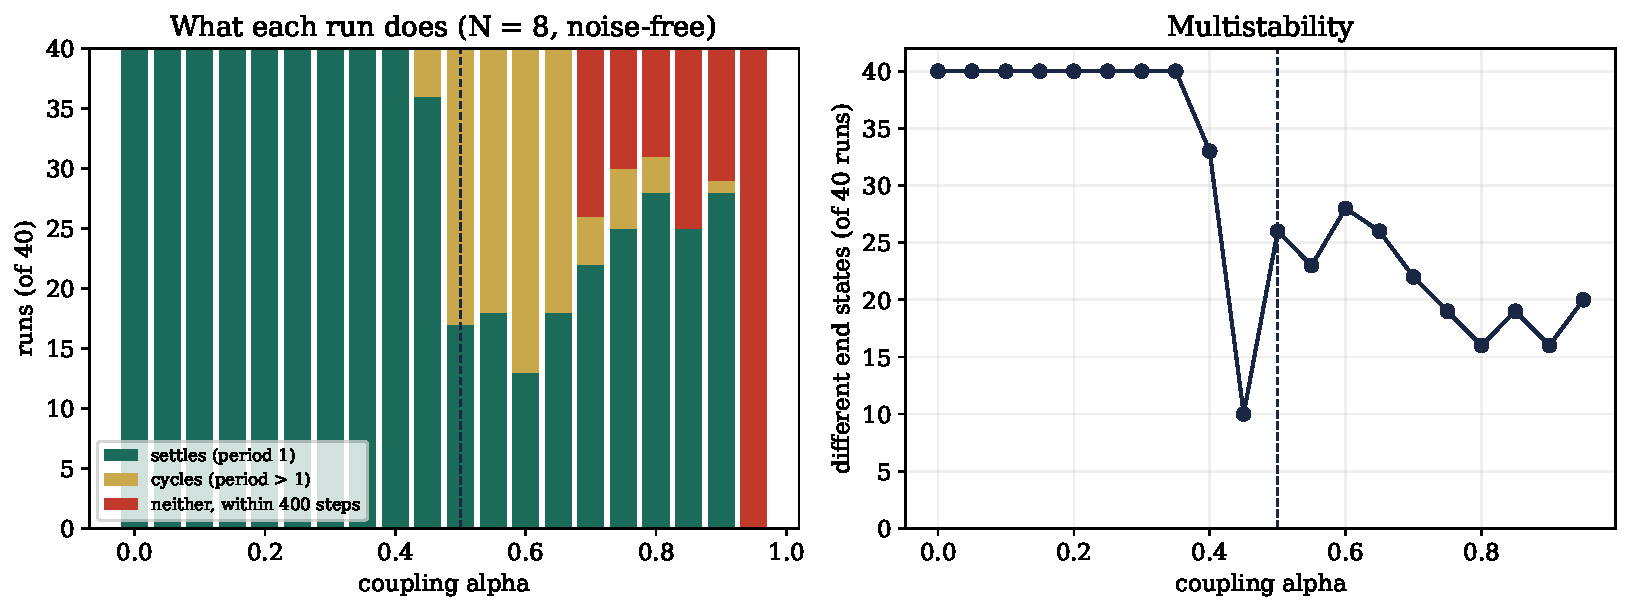
\includegraphics[width=\linewidth]{fig2_attractor_scan}
\caption{Left: what each of 40 runs does, by coupling. Right: number of different end states.}\label{fig:scan}
\end{figure}

Three regimes appear. For $\alpha\le0.35$ the model is multistable: every run settles, and every run settles
somewhere different. Settling is fast: at $\alpha=0.3$, after six steps each of 200 runs is within $1.5\%$ of its own
end state (Figure~\ref{fig:settle}), well inside version~2's bound of $27\%$. From $\alpha=0.42$ cycles appear, and for
$0.5\le\alpha\le0.65$ more runs cycle than settle. From $\alpha=0.7$ some runs neither settle nor repeat within 400
steps, and at $\alpha=0.95$ none do. The change near $\alpha\approx0.42$--$0.5$ is close to the threshold version~2
proposed, but it is a move from many resting states to cycles and irregular motion, not one state splitting in
two. Why it happens there is not proved here.

\begin{figure}[h]\centering
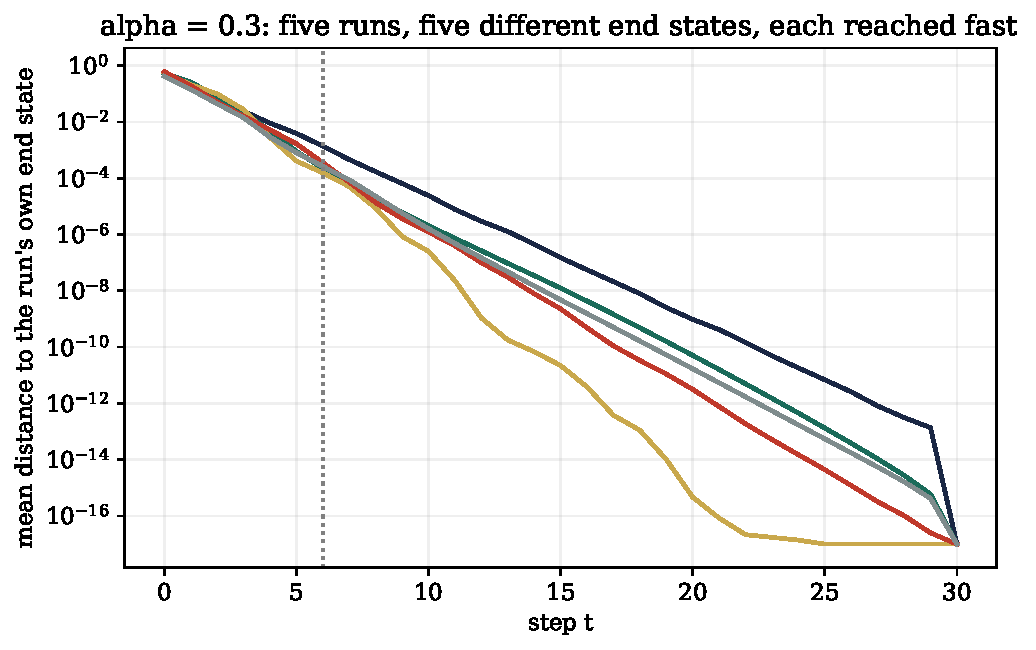
\includegraphics[width=0.72\linewidth]{fig3_settling}
\caption{$\alpha=0.3$: five runs, each approaching its own end state; the dotted line marks six steps.}\label{fig:settle}
\end{figure}

\begin{remark}[Interpretation]
Multistability is the feature the multi-orbit picture needs: separate runs, or separate clusters, can end in
separate stable states. The move to cycles as coupling grows is reminiscent of the switch between rest and
oscillation in stress-axis models \cite{Zarzer2013}, but the model has not been compared with any physiological
parameter, and the analogy is not a claim.
\end{remark}

\section{Lean~4 Verification}
The file \texttt{BioSwarmCheck.lean} defines $C$, $K_b$, $F_\alpha$, $U$ and $G$ exactly as in
Definition~\ref{def:G} and proves, with no \texttt{sorry} and only the axioms \texttt{propext},
\texttt{Classical.choice}, \texttt{Quot.sound} (Lean~4.32.0, Mathlib v4.32.0; 17 declarations audited):
\begin{center}\small
\begin{tabular}{@{}ll@{}}\toprule
Lean theorem & Statement\\\midrule
\texttt{C\_jumps} & Proposition~\ref{prop:jump} (the $\ell^1$ distances $1/500$ and $2$)\\
\texttt{four\_fixed\_points} & Proposition~\ref{prop:four}\\
\texttt{U\_norm} & Proposition~\ref{prop:norm}\\\bottomrule
\end{tabular}
\end{center}
The measurements of Section~4 are numerical and are not proved; \texttt{multi\_orbit\_bioswarm\_v3.py --check}
reproduces them.

\section{Open Questions}
\begin{enumerate}[leftmargin=2em,itemsep=2pt]
\item \textbf{The transition.} Why do cycles appear near $\alpha\approx0.42$, and how does the onset depend on $N$ and $b$?
\item \textbf{Counting attractors.} How many stable states are there for weak coupling, as a function of $N$? The runs suggest
very many (every one of 40 starts ends differently).
\item \textbf{Connectome data.} Fit coupling constants to the FlyWire weight matrix \cite{Dorkenwald2024} and compare with
module structure \cite{Schlegel2024}.
\item \textbf{Stress axis.} Relate the transition to measurable HPA parameters \cite{Zarzer2013}, or drop the analogy.
\end{enumerate}

\section{Corrections since Version 2}
(i) The Lipschitz constant $L(\alpha)=\tfrac12+|\alpha|$, the contraction for $|\alpha|<\tfrac12$ and the unique fixed
point are withdrawn (Propositions~\ref{prop:jump}, \ref{prop:four}). (ii) The pitchfork figure is withdrawn and replaced
by Figure~\ref{fig:scan} (Proposition~\ref{prop:norm}). (iii) The six-step bound $(4/5)^6$ is replaced by the measured
settling of Figure~\ref{fig:settle}. (iv) The Lean file is replaced by \texttt{BioSwarmCheck.lean}; version~2's file
stays in the record. (v) Reference [11] of version~2 is withdrawn and replaced by \cite{Zarzer2013}. (vi) The
dm$^3$ normalisation triple, which version~2 checked as arithmetic but did not use, is omitted.

\section*{Data and Code Availability}
Deposited with this PDF: \texttt{multi\_orbit\_bioswarm\_v3.tex}; \texttt{BioSwarmCheck.lean} and its axiom report;
\texttt{multi\_orbit\_bioswarm.py} (version~2 operators, unchanged) and \texttt{multi\_orbit\_bioswarm\_v3.py}
(measurements, figures, \texttt{--check}); \texttt{figures/} with \texttt{scan\_v3.csv}.

\begin{thebibliography}{9}
\bibitem{Grossi2026_MultiAgent} P.~Nogueira Grossi, ``Biological Transitions as Multi-Agent Realisations of the Generative Operator Pipeline in Topographical Orthogonal Generative Theory (TO/TOGT).'' G6 LLC. Zenodo: 10.5281/zenodo.19208015 (2026).
\bibitem{Grossi2026_Vol1} P.~Nogueira Grossi, \textit{Principia Orthogona, Volume One: The Mathematics of Generative Transitions}. G6 LLC. Zenodo: 10.5281/zenodo.19117400 (2026).
\bibitem{Dorkenwald2024} S.~Dorkenwald \textit{et al.}\ (FlyWire Consortium), ``Neuronal wiring diagram of an adult brain,'' \textit{Nature} \textbf{634}, 124--138 (2024). doi:10.1038/s41586-024-07558-y
\bibitem{Schlegel2024} P.~Schlegel \textit{et al.}, ``Whole-brain annotation and multi-connectome cell typing of \textit{Drosophila},'' \textit{Nature} \textbf{634}, 139--152 (2024). doi:10.1038/s41586-024-07686-5
\bibitem{Winding2023} M.~Winding \textit{et al.}, ``The connectome of an insect brain,'' \textit{Science} \textbf{379}, eadd9330 (2023). doi:10.1126/science.add9330
\bibitem{PerezCervera2019} A.~P\'erez-Cervera, T.~Seara, G.~Huguet, ``The uncoupling limit of identical Hopf bifurcations with an application to perceptual bistability,'' \textit{J.\ Math.\ Neurosci.}\ \textbf{9}, 7 (2019). doi:10.1186/s13408-019-0075-2
\bibitem{Zarzer2013} C.~A.~Zarzer, M.~G.~Puchinger, G.~K\"ohler, P.~K\"ugler, ``Differentiation between genomic and non-genomic feedback controls yields an HPA axis model featuring hypercortisolism as an irreversible bistable switch,'' \textit{Theor.\ Biol.\ Med.\ Model.}\ \textbf{10}, 65 (2013). doi:10.1186/1742-4682-10-65
\end{thebibliography}
\end{document}
